% -------------------------------------------------------------------
% 1. Инструменты и вводная
% -------------------------------------------------------------------

\lecture[17 августа 2026]{1}{Инструменты и теория}

\textbf{Дисклеймер.} В~этой инструкции описаны основные определения
и~собраны ссылки на~материалы для~обучения в~помощь начинающим
дизайнерам. Все~книги и~курсы авторы читали и~проходили
самостоятельно, поэтому информация предвзята, субъективна
и~не~является актуальным отражением положения дел в~индустрии.
На~момент написания авторы находились на~джуниор"=миддл"=позиции,
поэтому, пожалуйста, относитесь ко~всей информации ниже скептически
и~ищите дополнительные источники информации. Поиск и~проверка
информации~"--- ваш базовый навык как профессионала в~любой сфере,
особенно актуальный во~времена галлюционирующего ИИ~:-)

\begin{definition}[кто такой продуктовый дизайнер]
	Продуктовый дизайнер~"--- человек, использующий
	инструменты и~методологию дизайна при~работе над~цифровым
	продуктом и~влияющий на~его~развитие. 
\end{definition}

Продуктовый дизайнер отвечает за то, что~происходит в~продукте: проектирует
новые фичи, реагирует на~обратную связь пользователей и~бизнеса.
UX/UI-дизайнеры проектируют интерфейсы, а продуктовые~"--- исследуют,
анализируют, работают с пользователями и стейкхолдерами и только в последнюю
очередь~"--- проектируют элменты интерфейса. 

Ключевый термин в~работе продуктового дизайнера~"--- \textbf{метрики},
или~количественные показатели продукта. Существует большое количество метрик
для~оценки состояния продукта~"--- например, MAU, DAU, Retention, CTR. Каждая
метрика прямо или~косвенно отвечает на вопрос «что происходит с продуктом».

\begin{warning}
	Не все школы дизайна считают, что~продуктовый дизайнер обязан
	погружаться в~метрики. Тем не~менее, полезно знать хотя~бы
	некоторые из~них, чтобы говорить на~одном языке с~менеджерами
	продукта и~стейкхолдерами~"--- владельцами бизнеса. 
\end{warning}

Базовый минимум дизайнера:

% Делаем и элементы списка полужирным.~"--- Rikudo
\begin{enumerate}[{\bfseries 1.}]
	\item \textbf{Инструменты:} Фигма, Клод, ЧатЖПТ, Миджорни (базово). На~август
		2026 rода рекомендуем добавить Клод~Код, Фигма-агент и~Гитхаб.
		Желательно~"--- добавить как~минимум один инструмент для~работы с~растровой
		графикой и~видео (Фотошоп, Иллюстратор, Блендер, Афтер~Эффектс). Для начала
		хватит бесплатных видеоуроков с Ютуба и практических заданий.  

		Можно поспорить с~тем, нужна~ли в~2026~году работа с~Фотошопом, если есть
		Фотопеа и~Нано Банана. Мы гарантируем читателям задачу, на~которую
		в~какой-то момент не~хватит токенов или~понимания моделью вашей идеи.
		Фотошоп пригодится для~точечной, быстрой обработки растровых изображений,
		например, для~комментирования чужих работ.

	\item \textbf{Теория:} гештальт, композиция, типографика, цвет, графический
		дизайн, анимация, интерфейсы, пользовательский опыт.

	\item \textbf{Продуктовый подход:} метрики, СJM, JTBD, исследования.  

	\item \textbf{Софт-скиллы:} переговоры, управление, обратная связь,
		работа в~команде. 
\end{enumerate}

Всё перечисленное выше можно и~нужно уложить в~единую систему обучения.
Рекомендуем одну из~готовых систем:

\begin{enumerate}
	\item Школа дизайнеров (Бюро Горбунова)~"--- фундаментальные знания
		о~типографике, интерфейсах, редактуре и~переговорам. Советуем изучить
		\href{https://bureau.ru/school/designers}{программу школы и~список
		рекомендуемых книг.} Учёба потребует сил, но~подойдёт и~новичкам,
		и~практикующим дизайнерам.

	\begin{figure}[h]
  		\centering
			% Костыль: img/
  		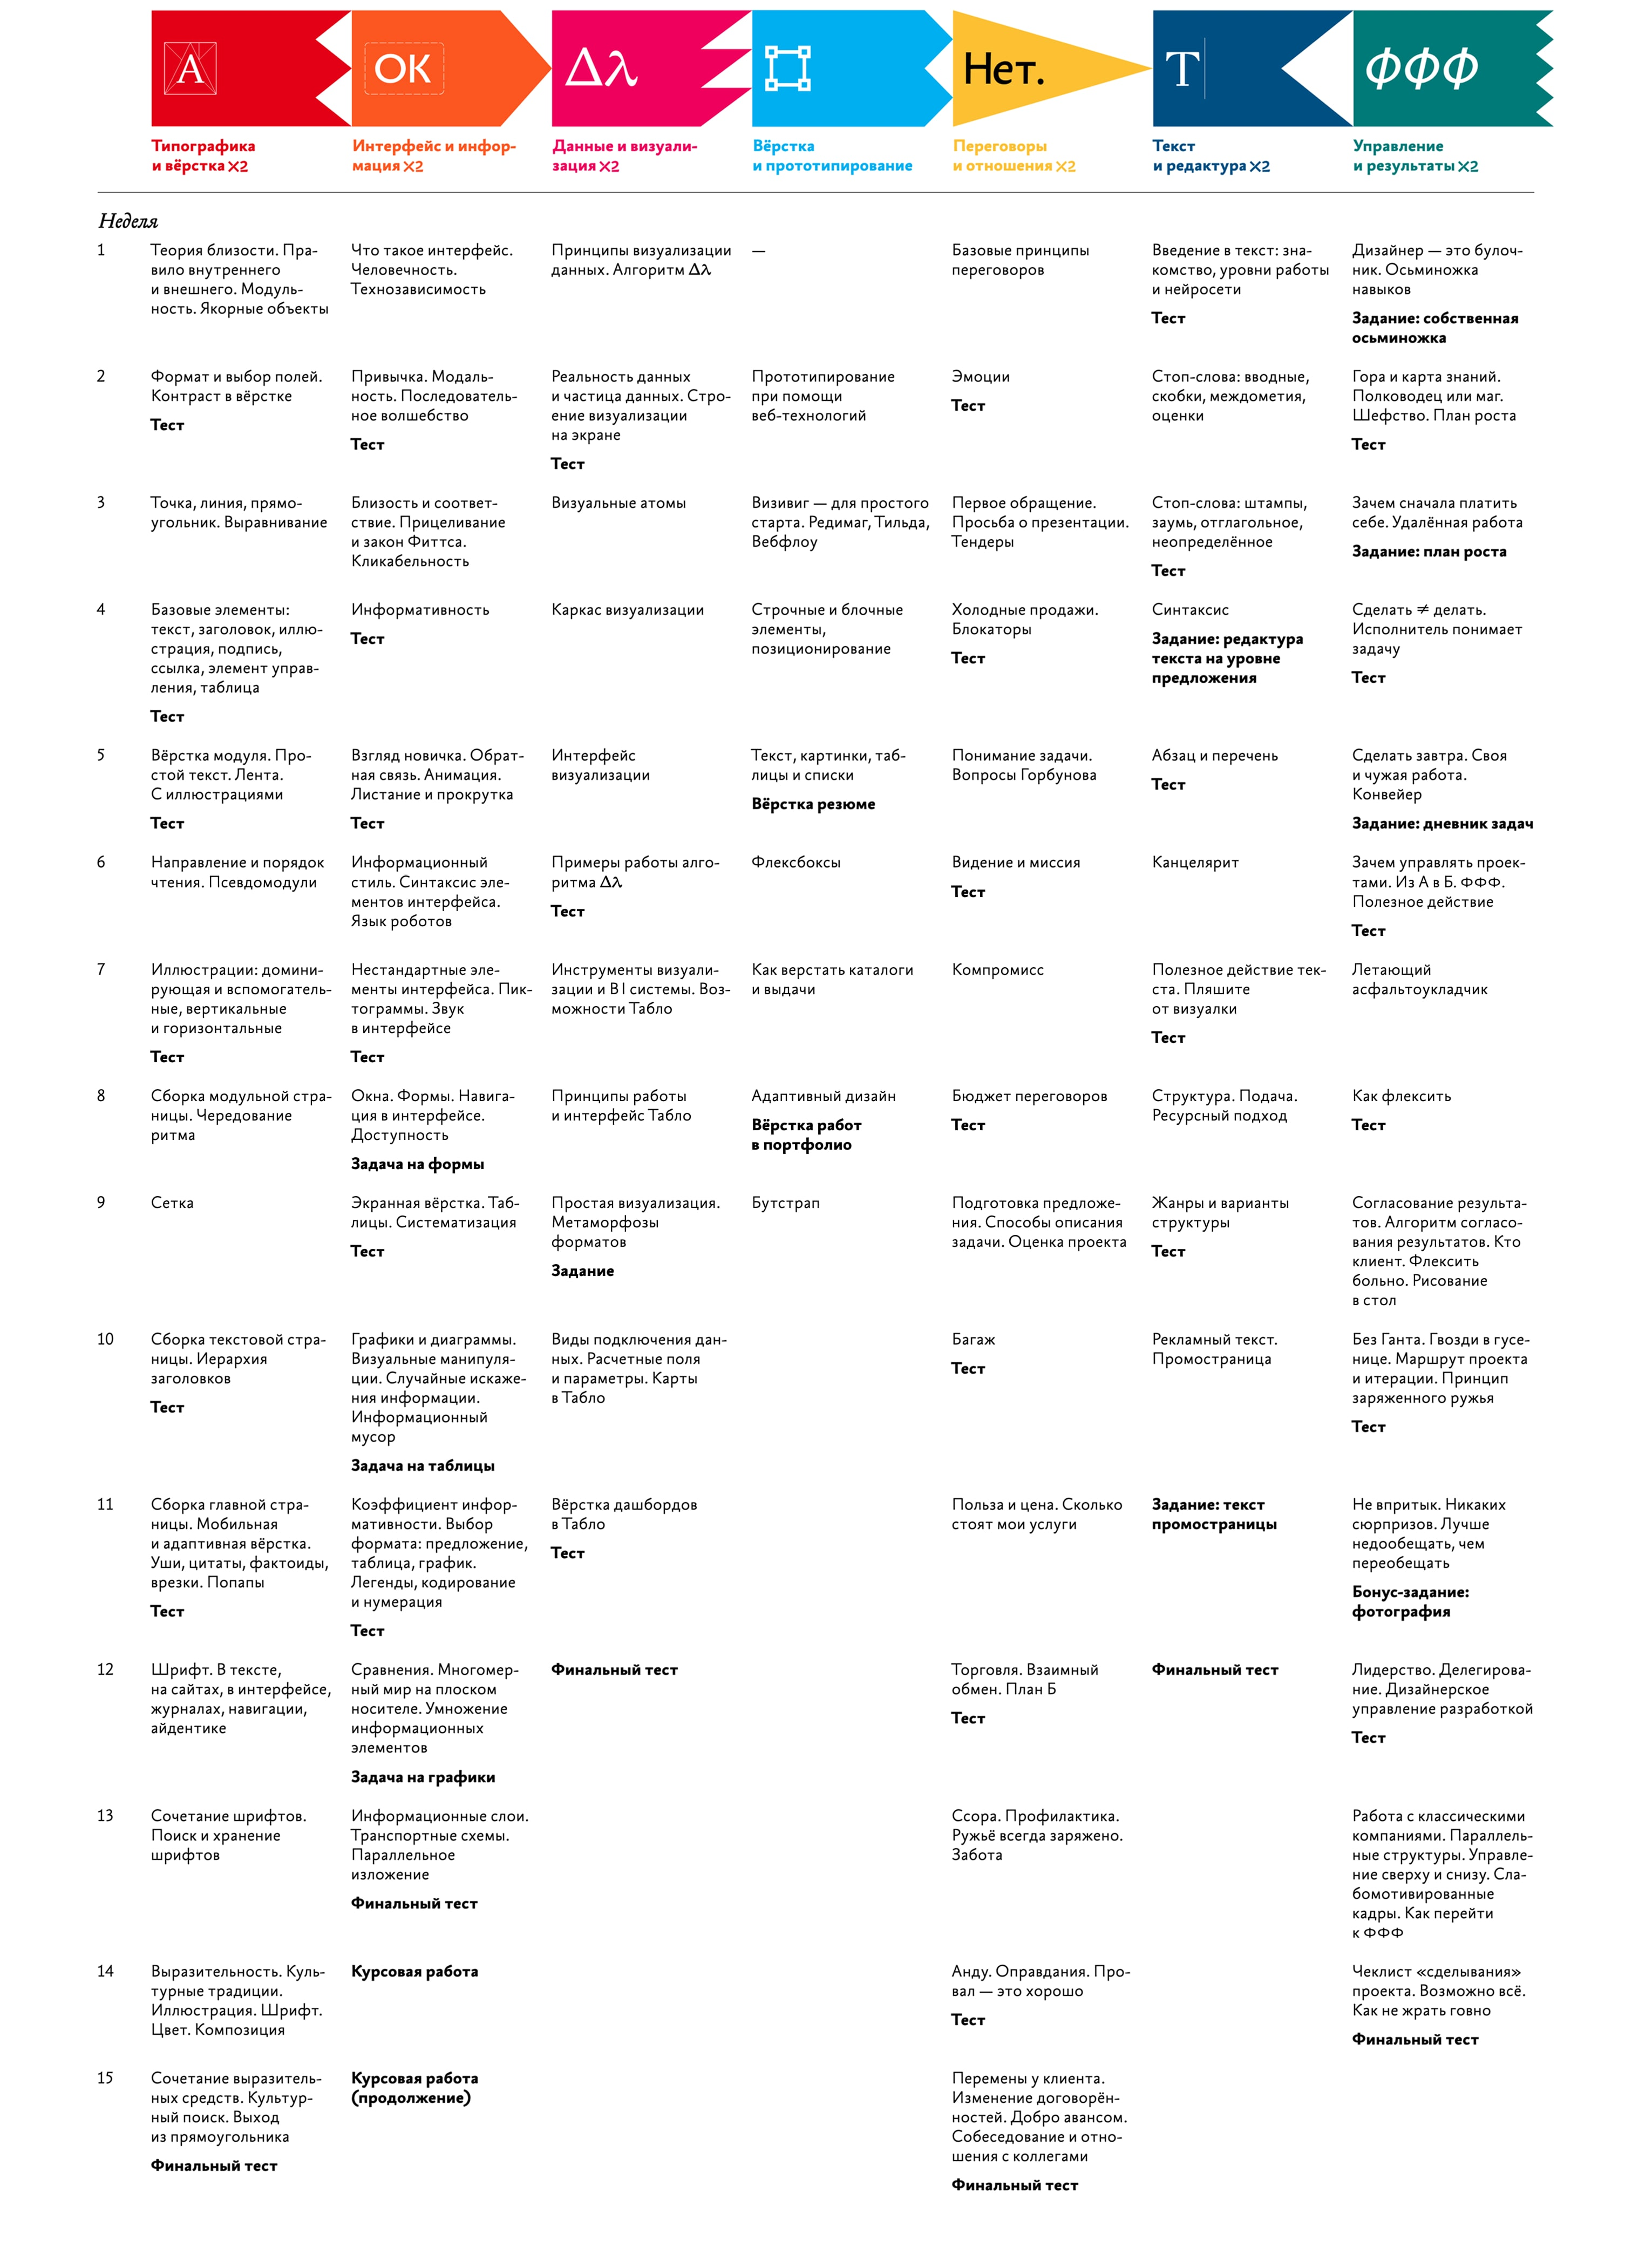
\includegraphics[width=\textwidth]{img/program} 
			\caption{Дисциплины и~темы, которые проходят в~Школе дизайнеров}
	\end{figure}

	%
\includegraphics[width=\textwidth]{program} 

	\begin{tip}
		В школе есть бесплатные места, на которые поступают по~конкурсу. Успешно
		закончившим все три ступени могут предложить работу в~Бюро и~в~компаниях"=партнёрах.
	\end{tip}

	\item Как стать дизайнером (Женя Арутюнов, Интуиция)~"---
		\href{https://intuition.team/ru/design-roadmap}{подробный список тем
		с~порядком их~изучения} Подойдет для учёбы в~своем темпе и~для~углубления
		знаний по конкретным вопросам. Если сомневаетесь в~своём интересе к
		дизайну, советуем начать отсюда.

	\item Superpowered UX/UI. (cтудия PINKMAN)"---
		\href{https://wannabe.ru/design/superpowered}{курс, который постоянно
		обновляет программу и инструменты} Не подойдёт, если вы только начали
		работать в~Фигме или сомневаетесь в~своём направлении. Плюс~"--- актуальные
		знания. Вы~будете пользоваться последними инструментами, знать, как
		работуют практикующие дизайнеры исможете выстроить дизайн-процесс. 

\end{enumerate}


% \begin{takeaways}
% 	\begin{itemize}
% 		\item Вывод «А»;
% 		\item Вывод «Б»;
% 		\item Вывод «В»;
% 	\end{itemize}
% \end{takeaways}

% vim:ts=2:sw=2:tw=68
